\renewcommand*{\arraystretch}{1.1}

\subsection{Interactive / delete / 1}
\label{sec:interactive-delete-01}

% change \emph{} to use sans-serif font
\let\oldemph\emph
\renewcommand{\emph}[1]{{\footnotesize \sf #1}}

\renewcommand{\currentQueryCard}{1}
\marginpar{
	\raggedleft
	\vspace{0.22ex}

	\queryRefCard{interactive-delete-01}{ID}{1}\\
	\queryRefCard{interactive-delete-02}{ID}{2}\\ 
	\queryRefCard{interactive-delete-03}{ID}{3}\\
	\queryRefCard{interactive-delete-04}{ID}{4}\\
	\queryRefCard{interactive-delete-05}{ID}{5}\\
	\queryRefCard{interactive-delete-06}{ID}{6}\\
	\queryRefCard{interactive-delete-07}{ID}{7}\\
	\queryRefCard{interactive-delete-08}{ID}{8}\\
}


\noindent\begin{tabularx}{\queryCardWidth}{|>{\queryPropertyCell}p{\queryPropertyCellWidth}|X|}
\hline
query & Interactive / delete / 1 \\ \hline
%
title & Remove person \\ \hline
%
% pattern & \centering 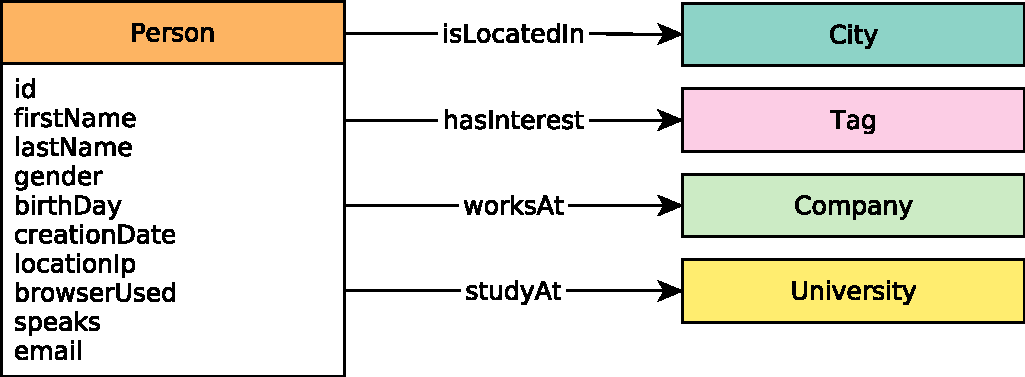
\includegraphics[scale=\patternscale,margin=0cm .2cm]{patterns/interactive-update-01} \tabularnewline \hline
%
desc. & Remove a \emph{Person} \textbf{node} and it's incident \textbf{edges} (\emph{isLocatedIn}, \emph{studyAt}, \emph{workAt}, \emph{hasInterest}, \emph{likes}, \emph{knows}, \emph{hasMember}, \emph{hasModerator}, \emph{hasCreator}). The removal of a \emph{Person} removes all \emph{Forum} they are moderator of and all messages they have posted in other forums. 
\\ \hline
%
params & \innerCardVSpace{\begin{tabularx}{\attributeCardWidth}{|>{\paramNumberCell}c|>{\varNameCell}M|>{\typeCell}m{\typeWidth}|Y|} \hline $\mathsf{1}$ & Person.id & ID & \texttt{forumId} \\ \hline
\end{tabularx}}\innerCardVSpace \\ \hline	
%	
comments &
\begin{itemize}
  \item Removal of a person can (1) remove all associated posts/comments/forum nodes or (2) just the person node. GDPR is a valid argument for (1). Approach (2) could lead to problems with read queries, driver gathering parameters for short reads and inadvertently impose implementation decisions for implementors. 
\item Removal of a person removes forums of type ``personal walls'' and ``image albums'' not ``groups'', which can continue if even the founder has left the network. The hasModerator edge must transition to an existing person node in the network, two approaches to assigning a new moderator were discussed: (1) choose member at random from the set of existing group members or (2) the member with the oldest group join date becomes the moderator.   
\item Removal of a person removes all posts/comments they are creator of this could result in the removal of a comment in the middle of a thread. 
\end{itemize}
 \\ \hline
%
% 
%
%
\end{tabularx}
\queryCardVSpace

% change \emph back to the old one
\let\emph\oldemph


